\pagebreak
\section{Situation in POP-C++}



In the current version of POP-C++, several connections are made between interfaces and brokers. These connections are the following : 
\begin{enumerate}
\item JobMgr to JobMgr : a JobMgr contacts other JobMgr to register itself to them.
\item PSN to PSN : The POPCSearchNode (PSN) contacts other PSN to discover resources.
\item Object Interface to Object Broker : The interface of a parallel object contacts its broker to perform method calls.
\item Parallel object to Application Services : The parallel object might contact the Application Services to use the Remote Log Service, the Object Monitor Services ...
\end{enumerate}

Figure \ref{fig:crt_sit} shows the communications established during the execution of a POP-C++ application with two parallel objects. This application is using five remote connections during its execution. The local communications will not be secured as they do not send data over the network.

\begin{figure}[ht]
	\caption{Current situation in POP-C++}
  	\centering
	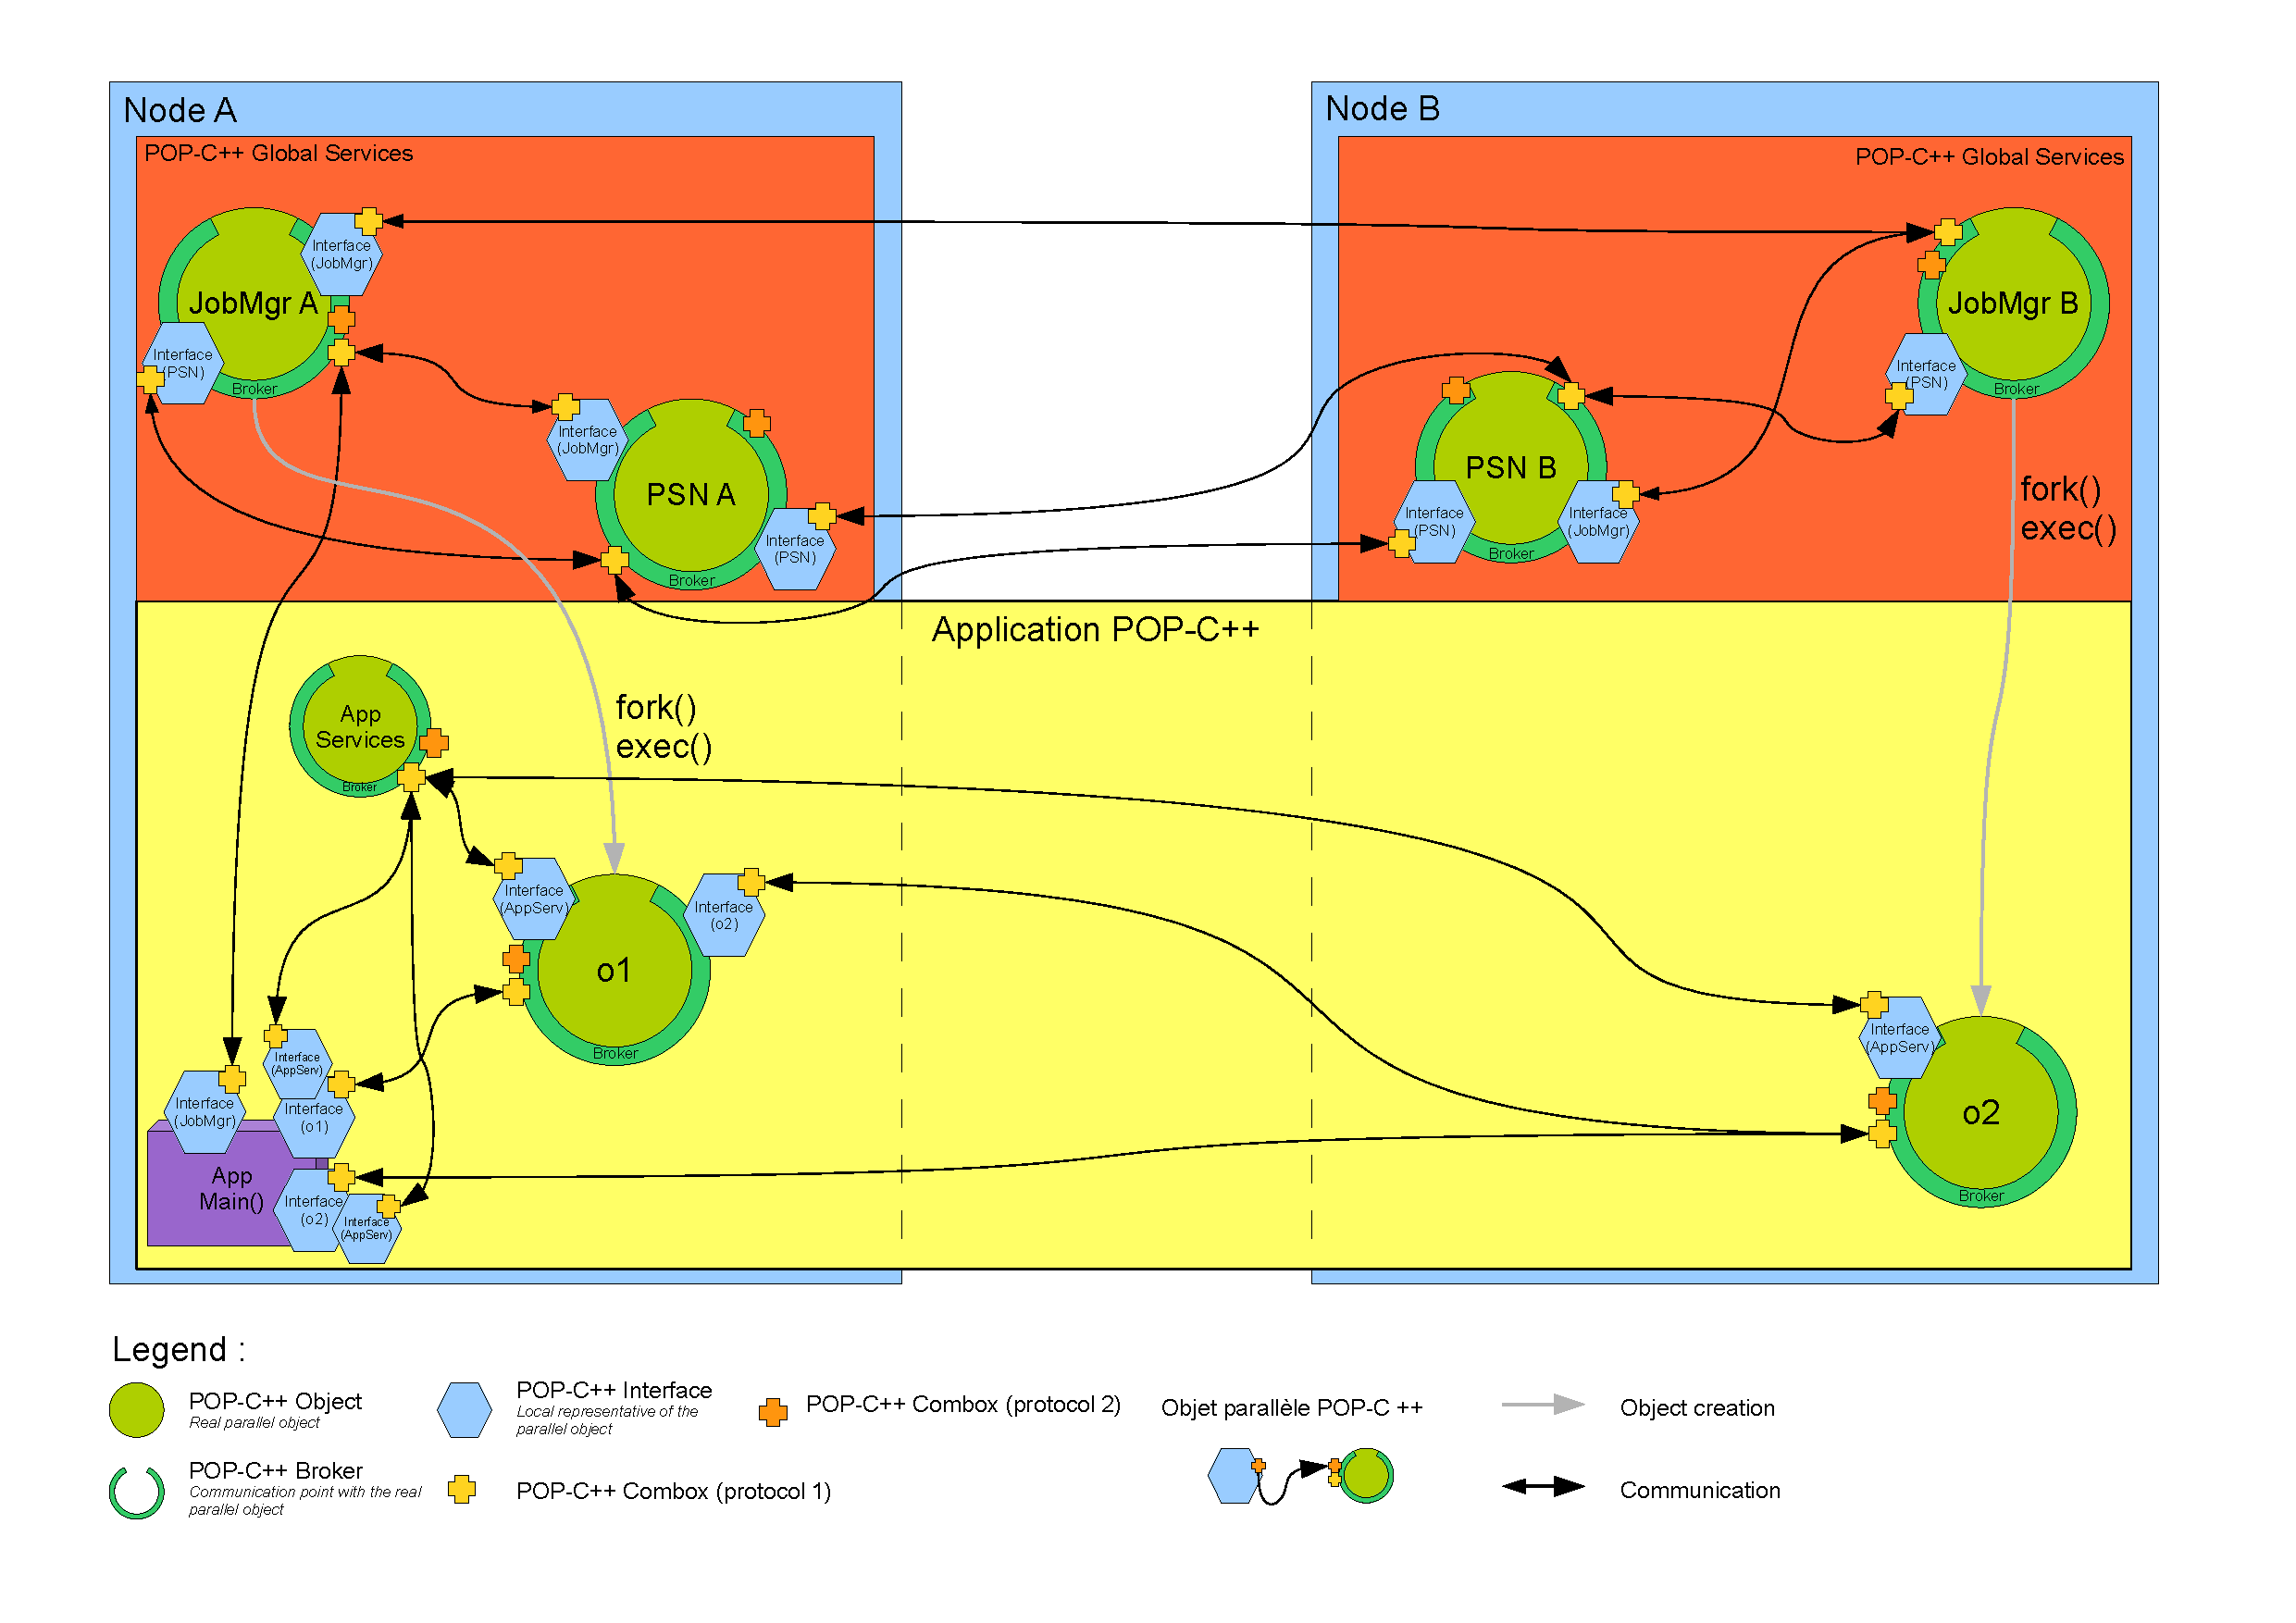
\includegraphics[width=1.0\textwidth]{../popc_crt_situation.pdf}
	\label{fig:crt_sit}
\end{figure}

\textit{NOTE:} The connection is always initiated from an interface to a broker.
\pagebreak



The new implementation of POP-C++ using SSH Tunnelling must create a SSH Tunnel between each remote connection. As shown in Figure\ref{fig:final_sit}, at least four SSH Tunnels are needed to secure the same application. In fact, each parallel objects are listening to different ports. Due to this fact, different SSH tunnels are needed. The interface will connect itself to a local address on a random defined port and the SSH tunnel will automatically redirect this connection to the right remote address and port. All the data sent over the network will be encrypted by the SSH protocol.
\begin{figure}[ht]
	\caption{Final situation in POP-C++}
  	\centering
	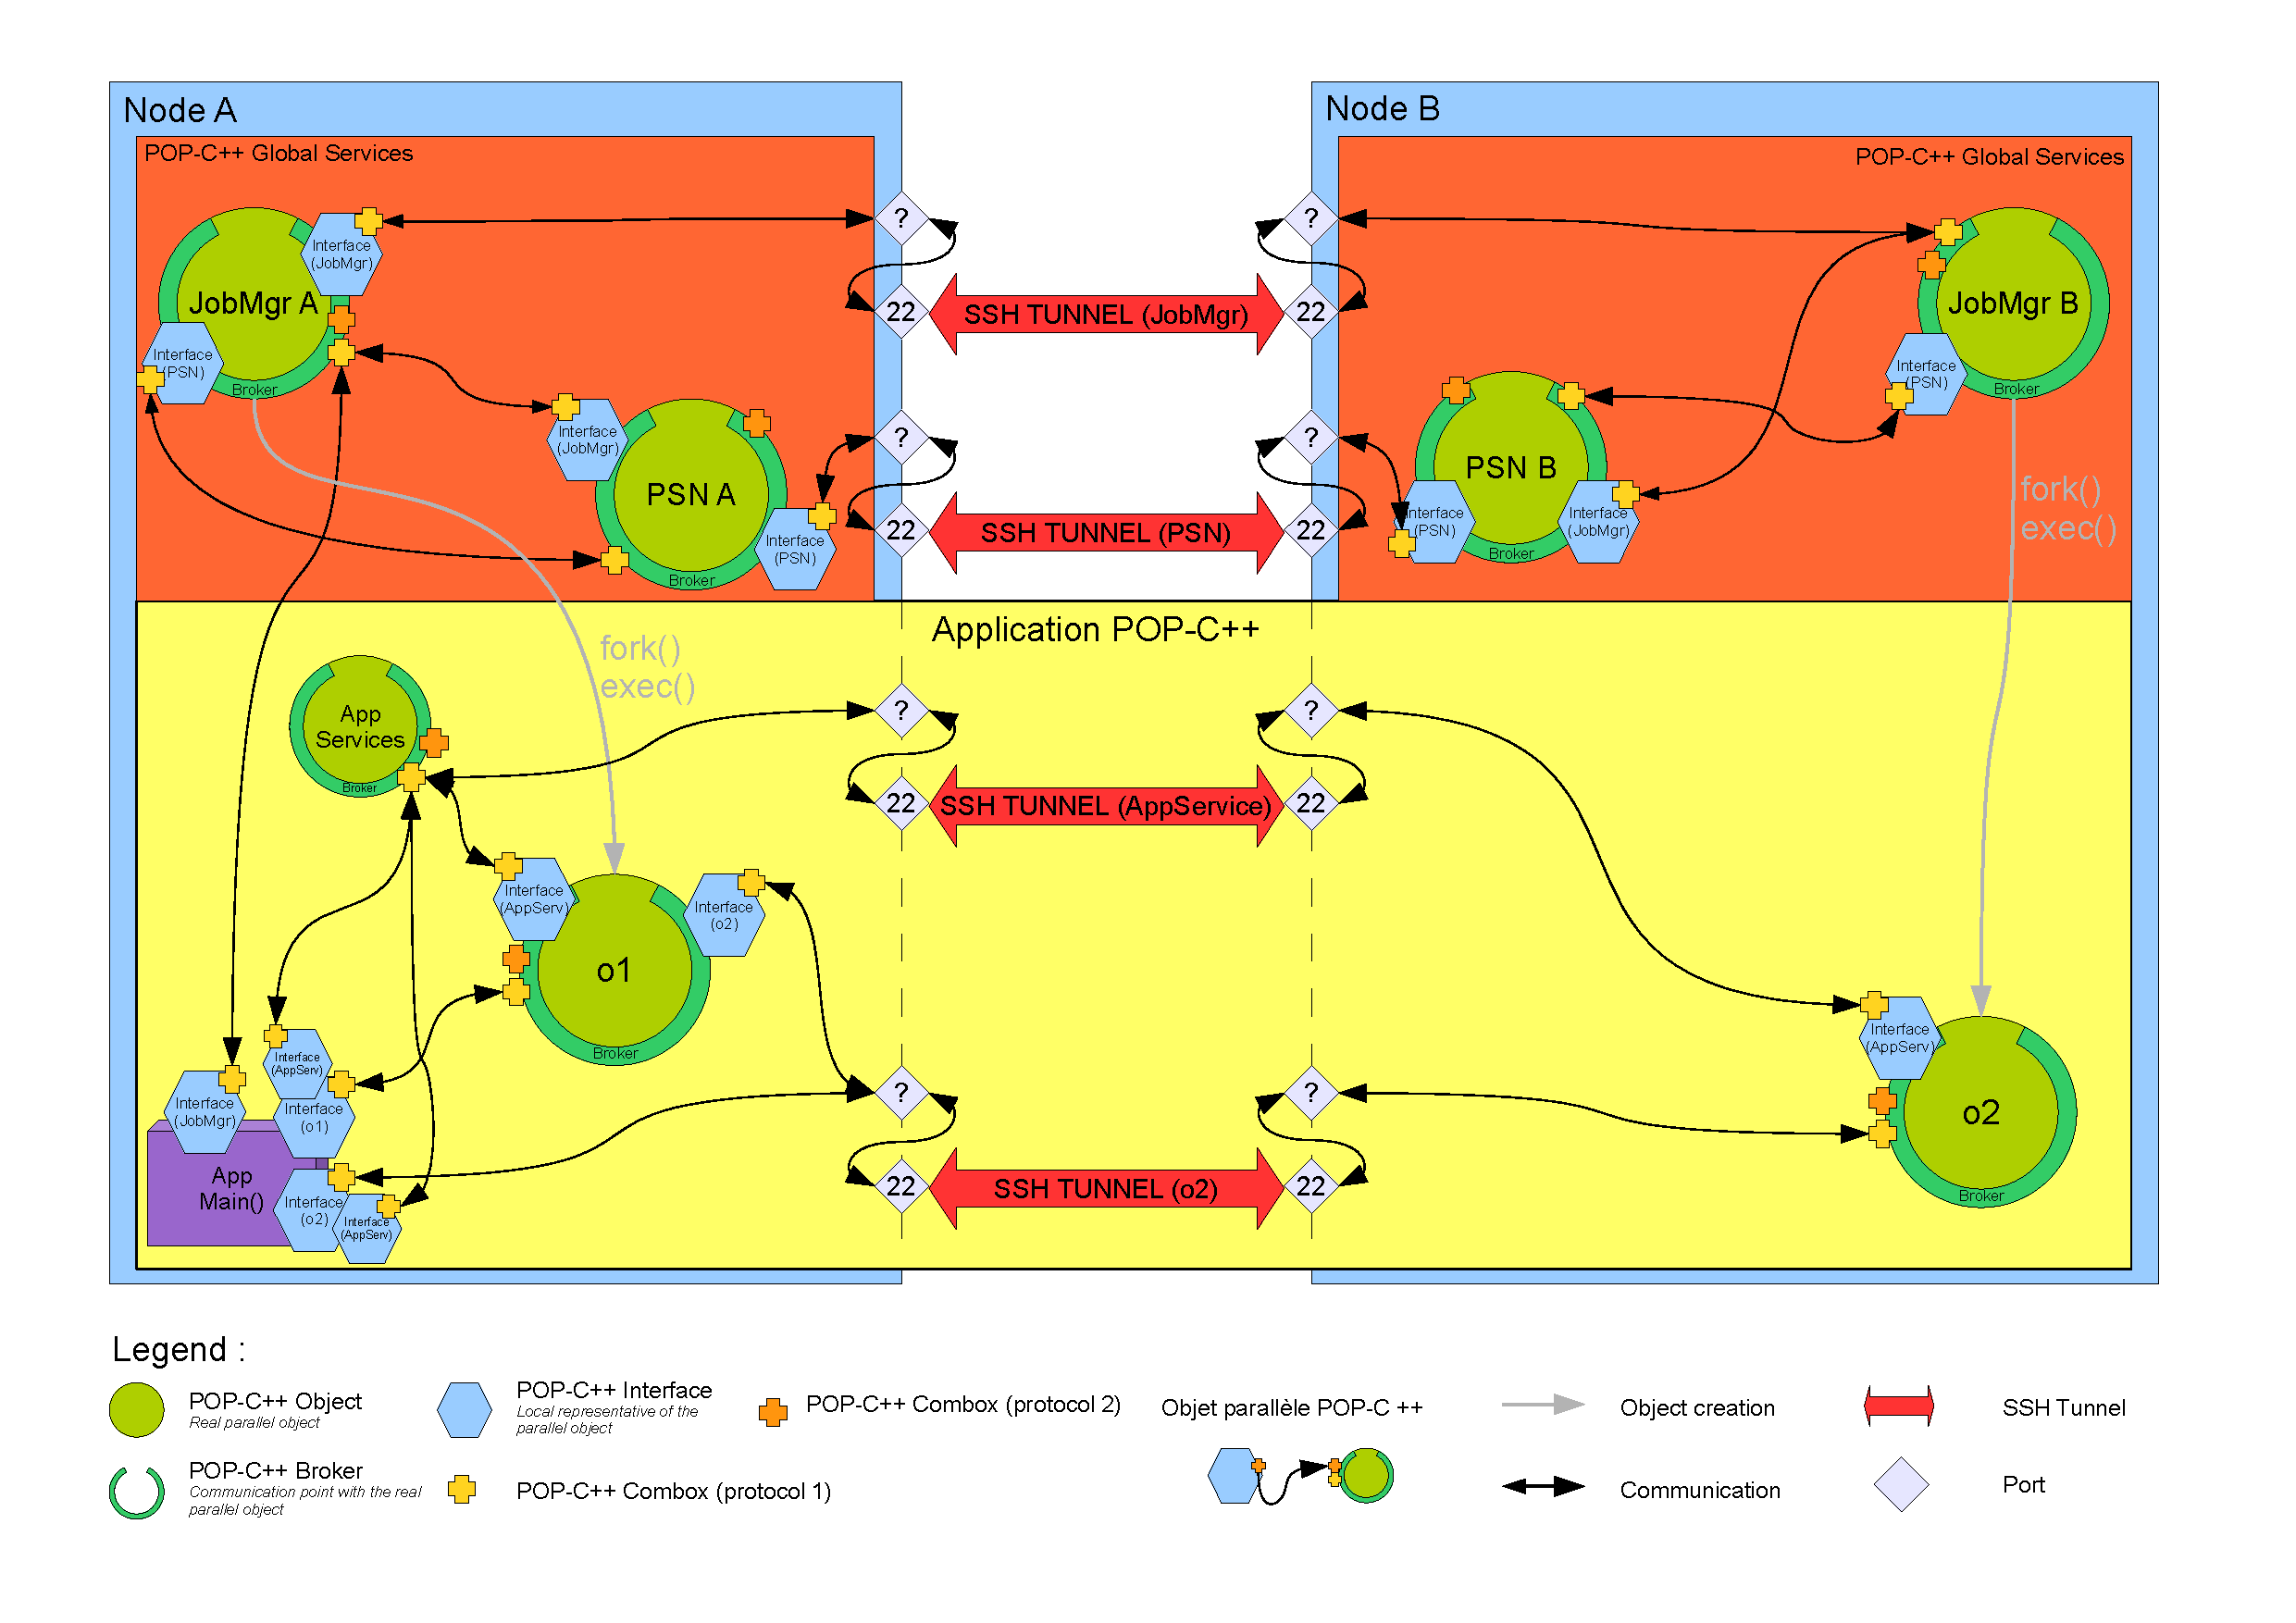
\includegraphics[width=1.0\textwidth]{../popc_final_situation.pdf}
	\label{fig:final_sit}
\end{figure}\vspace{2cm}
\pagebreak